\documentclass[varwidth=241.14749pt,class=acmart,sigconf,nonacm]{standalone}
%\documentclass[varwidth=506.295pt,class=acmart,sigconf,nonacm]{standalone}
\providecommand{\paperroot}{..}

% all packages used by figures, global tikz options, etc. go here.

\usepackage{tikz}

\tikzset{>=stealth}

% all time plots ideally share the same dimensions
\newcommand{\timeaxis}{
	\draw[->] (18,0) -- (20+9/12,0);
	\foreach \year in {18,19,20} {
		\draw (\year,-15pt) node [right, inner ysep=0] {\small20\year~$\rightarrow$};
		\foreach \imonth/\month in {0/J,1/F,2/M,3/A,4/M,5/J,6/J,7/A,8/S,9/O,10/N,11/D}{
			\pgfmathparse{(\year > 18 || \imonth >= 0) && (\year < 20 || \imonth < 9)}
			\ifnum \pgfmathresult > 0
				\draw (\year + \imonth/12,0)++(1/24,0) node [below] {\footnotesize \month};
					\draw (\year + \imonth/12,0) -- ++(0,-3pt); 
			\fi
		}
		\draw (\year,0) -- ++(0,-6pt); 
	}
}
\begin{document}
\begin{figure}
	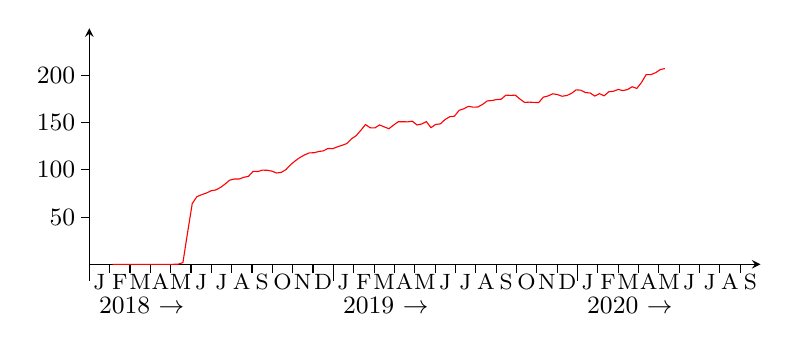
\begin{tikzpicture}[y=.012cm,x=3.1cm]
		
		% axes
		\timeaxis
		\draw[->] (18,0) -- (18,250);
		\foreach \y in {50,100,150,200}{
			\draw (18,\y) -- node [left] {\small\y} ++(-3pt, 0);
		};
		
		% plot data
		% use scopes to change colors or call custom commands defined here from the data file, but keep styling out of data.
		\begin{scope}[red]
			% These files should really only contain _individual_ tikz plot lines or \providecommands.
% It is better to put different plot lines in different files and then use \foreach in tikz,
% this allows you to toggle lines without rerunning analyses.
%
%
% For time plots specifically, representing dates as year.share-of-year floats gives you most flexibility.
% Here is some overengineered Python code:
%
% from datetime import date, datetime
% from typing import Union
% import sys
%
% def date_to_float(x: Union[date, datetime]) -> float:
%     full_year = date(x.year + 1, 1, 1) - date(x.year, 1, 1)
%     if isinstance(x, datetime):
%         elapsed = x - datetime(x.year, 1, 1)
%     else:
%         elapsed = x - date(x.year, 1, 1)
%     return x.year - 2000 + elapsed / full_year
%
% x = date.fromisoformat(sys.argv[1])
% print(f"{date_to_float(x)=:g}")
\draw (18.0959, 0) -- (18.1151, 0) -- (18.1342, 0) -- (18.1534, 0) -- (18.1726, 0) -- (18.1918, 0) -- (18.211, 0) -- (18.2301, 0) -- (18.2493, 0) -- (18.2685, 0) -- (18.2877, 0) -- (18.3068, 0) -- (18.326, 0) -- (18.3452, 0) -- (18.3644, 0.142857) -- (18.3836, 1.85714) -- (18.4027, 33.5714) -- (18.4219, 64.4286) -- (18.4411, 71.7143) -- (18.4603, 73.7143) -- (18.4795, 75.4286) -- (18.4986, 77.8571) -- (18.5178, 78.7143) -- (18.537, 81.2857) -- (18.5562, 85) -- (18.5753, 89.1429) -- (18.5945, 90.2857) -- (18.6137, 90.2857) -- (18.6329, 92.1429) -- (18.6521, 93.1429) -- (18.6712, 98.4286) -- (18.6904, 98.2857) -- (18.7096, 99.7143) -- (18.7288, 99.5714) -- (18.7479, 98.7143) -- (18.7671, 96.7143) -- (18.7863, 97.2857) -- (18.8055, 100.286) -- (18.8247, 105.429) -- (18.8438, 109.571) -- (18.863, 113.143) -- (18.8822, 115.857) -- (18.9014, 118) -- (18.9205, 118.143) -- (18.9397, 119.429) -- (18.9589, 120.143) -- (18.9781, 122.714) -- (18.9973, 122.429) -- (19.0164, 124.429) -- (19.0356, 126) -- (19.0548, 127.857) -- (19.074, 132.857) -- (19.0932, 136.143) -- (19.1123, 141.857) -- (19.1315, 148) -- (19.1507, 144.571) -- (19.1699, 144.429) -- (19.189, 147.571) -- (19.2082, 145.571) -- (19.2274, 143.571) -- (19.2466, 147.429) -- (19.2658, 151) -- (19.2849, 151) -- (19.3041, 150.857) -- (19.3233, 151.571) -- (19.3425, 147.571) -- (19.3616, 148.571) -- (19.3808, 151.143) -- (19.4, 144.714) -- (19.4192, 148.143) -- (19.4384, 148.714) -- (19.4575, 153.286) -- (19.4767, 156.286) -- (19.4959, 156.857) -- (19.5151, 163) -- (19.5342, 164.714) -- (19.5534, 167.286) -- (19.5726, 166.429) -- (19.5918, 166.571) -- (19.611, 169.286) -- (19.6301, 173) -- (19.6493, 173.429) -- (19.6685, 174.429) -- (19.6877, 174.857) -- (19.7068, 179.143) -- (19.726, 178.857) -- (19.7452, 179.143) -- (19.7644, 175) -- (19.7836, 171.429) -- (19.8027, 171.714) -- (19.8219, 171.429) -- (19.8411, 171.286) -- (19.8603, 177) -- (19.8795, 178.286) -- (19.8986, 180.571) -- (19.9178, 179.714) -- (19.937, 178) -- (19.9562, 178.714) -- (19.9753, 181) -- (19.9945, 184.714) -- (20.0137, 184.429) -- (20.0328, 181.857) -- (20.0519, 181.429) -- (20.071, 178.143) -- (20.0902, 180.714) -- (20.1093, 178.429) -- (20.1284, 182.714) -- (20.1475, 183.286) -- (20.1667, 185.143) -- (20.1858, 184) -- (20.2049, 185) -- (20.224, 188) -- (20.2432, 186.286) -- (20.2623, 192.571) -- (20.2814, 200.857) -- (20.3005, 200.857) -- (20.3197, 202.857) -- (20.3388, 206.143) -- (20.3579, 207.286);
;
		\end{scope}
	\end{tikzpicture}
	\caption{Example Figure}
	\label{fig:example}
\end{figure}
\end{document}